\section{Oddities}
\label{sec-oddities}

We now present some of the oddities in the \textit{Twilio} ecosystem that we discovered during our study. First, as dicussed in section \ref{sec-twilioecoandprotocolstudy}, \textit{Twilio} charges twice for making a single outgoing call. We discovered this from the call logs available in the Twilio user portal. On first seeing this, we thought this was problem in the VoIP service code that we developed. But it turns out that even after using the code examples from Twilio developer forums, we were still observing this behavior. It should be noted that we built our VoIP service on top of a single \textit{Twilio number}. Second, we noticed that some applications may require \texit{ordered} message delivery for the messages that they try to send through \textit{Twilio} APIs. For example, a message based query system will require that the messages sent are delivered to the mobile phone in the same order. We understand that the telephone service provider can also reorder messages when delivering them. We understand that \textit{Twilio} does not provide any guarantee as such for ordered message delivery. But we wanted to measure to what extent the messages can be reordered. 

\begin{figure*}[t!] \centering
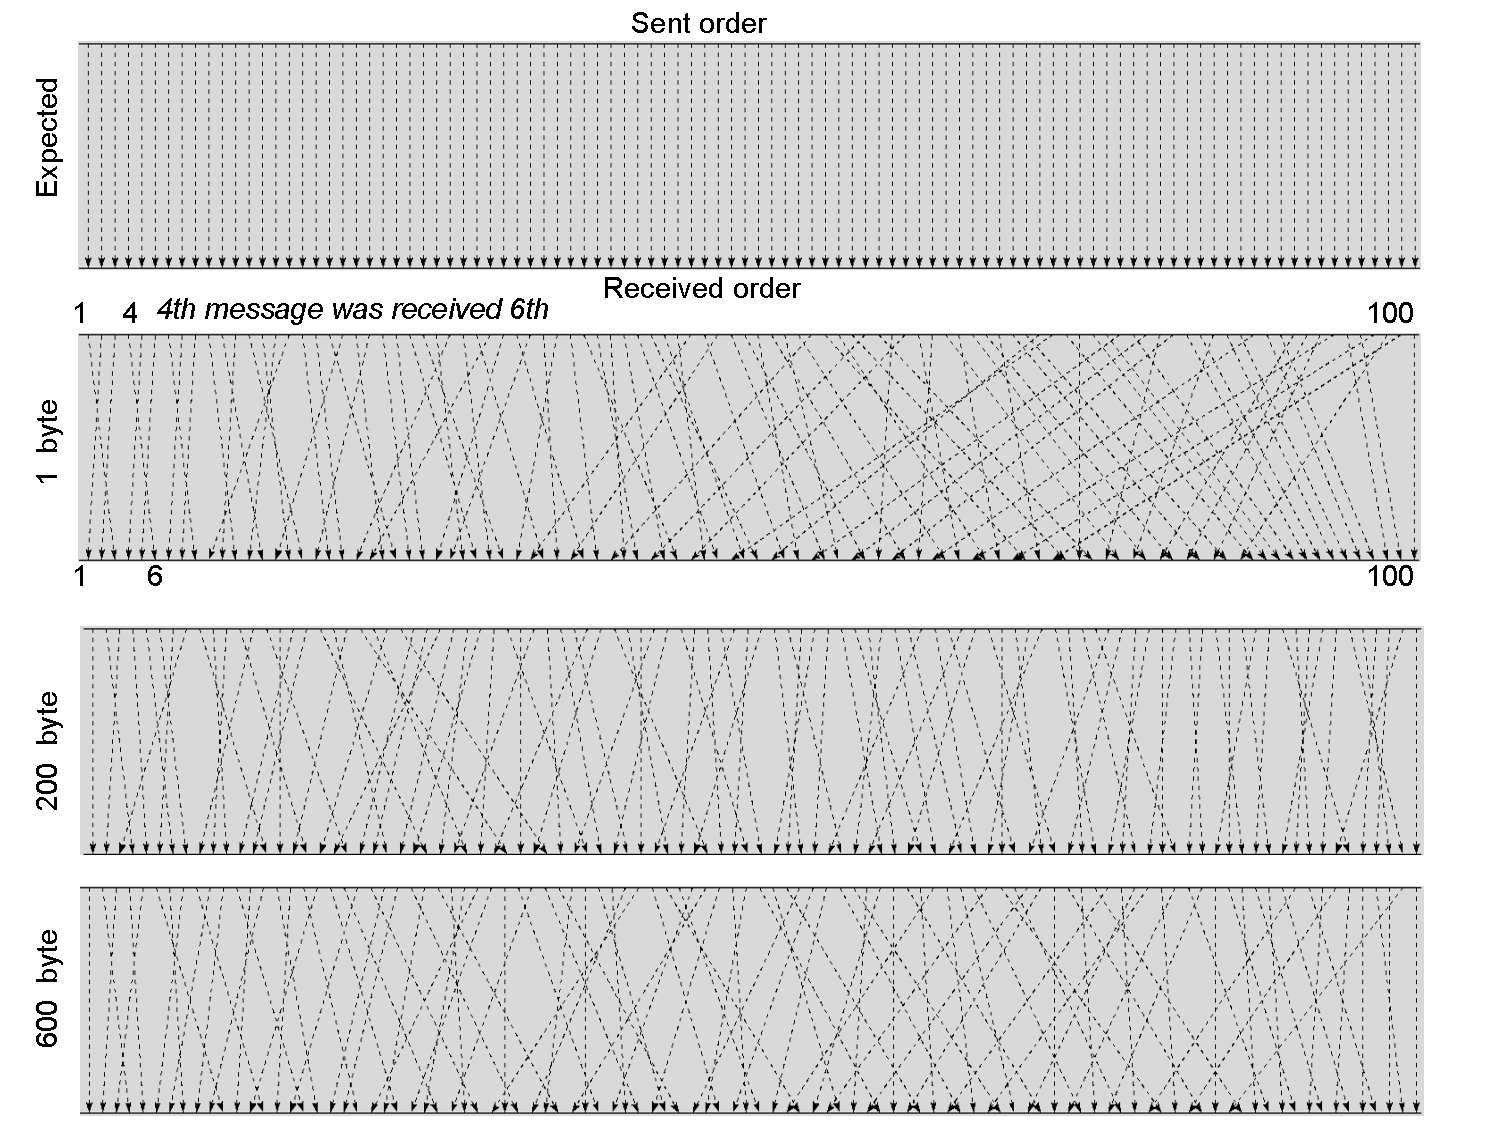
\includegraphics[width=\textwidth]{figs/reordering.pdf}
\caption{\textbf{SMS reordering} {\footnotesize\textit{
The figure shows the extent to which messages can get reordered. The top line in each strip denotes the sent order and the bottom line denotes the received order. The top most strip shows the ideal message delivery behavior. The second strip shows the reorderings that happened when 100 one byte messages were sent. The third strip shows the same for 200 byte messages and the last strip for 600 byte messages. Note that the sent time is identified from the \textit{sent timestamp} from the resource store so it represents the time for nearest upstream telephone carrier network to acknowledge the message was received and will be sent to the phone. 
}}}
\label{fig:reordering}
\end{figure*}


Figure {\ref{fig:reordering}} shows the message reorderings that can happen. It is understandable that \textit{Twilio} does not itself provide ordered message delivery. Application developers who develop on the \textit{Twilio} platform should be aware of this and should use suitable application level techniques to solve this issue. For example, the application use a label denoting the position of the message in the sequence. 

Third, we injected few faults into some parts of the system and observed how \textit{Twilio} reacts to these corner cases. For example we tested cases where in the \textit{TwiML} response returned by out VoIP server was malformed, unacceptably large, corrupted etc. We noted that the fault handling mechanisms were not uniform across all error scenarios. For example, if the \textit{TwiML Say verb} contained content greater than 4096 bytes, the call was placed but an error message was delivered to the attendee. On a different scenario when there are nested \textit{say} verbs in the \textit{TwiML} response, then a blank call was placed to the attendee. We are barely scratching the surface in terms of fault injection. We strongly believe that much better extensive techniques can be developed to analyse all the possible error conditions in the service.  

Fourth, during our study we observed a weird behavior in the \textit{Twilio Python client v3.66} library. We observed that when a client script tried to queue a call or a message using the \textit{create()} API, there was a HTTP level auth failure that was happening before the actual sequence of packets that were happening between the client and the \textit{Twilio} server. On further investigation and debugging, we found that the client was not passing the \textit{Auth Token} and \textit{Account SID} when the first REST API call is made to the server. Then the exception is handled and then the required credentials are passed onto the server for the subsequent REST API calls. We noted that this unwanted auth failure wastes 6 RTTs. We also believe that this can be easily optimized in the client library. 

\begin{figure*}[ht!] \centering
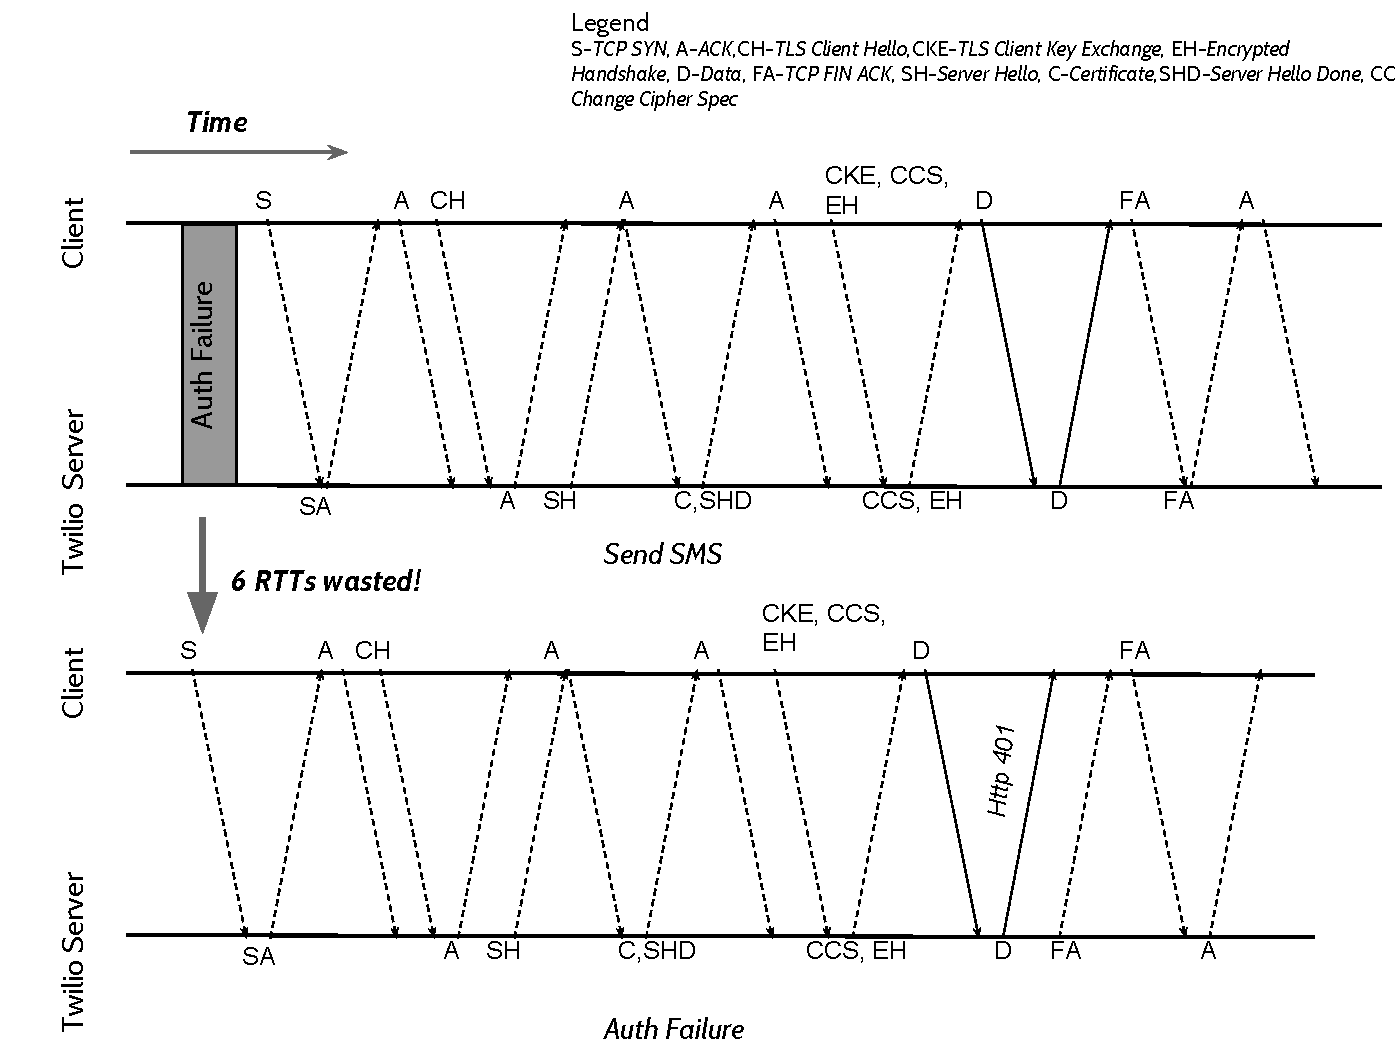
\includegraphics[width=\textwidth]{figs/authfailure.pdf}
\caption{\textbf{Packet analysis for creating automated SMS} {\footnotesize\textit{
The figure shows the sequence of packets exchanged between the client and the server when the client script tries to create a message.
}}}
\label{fig:authfailure}
\end{figure*}

Figure {\ref{fig:reordering}} explains this client library behavior. 